

\section{System Architecture}

\begin{figure}[ht!]
\centering
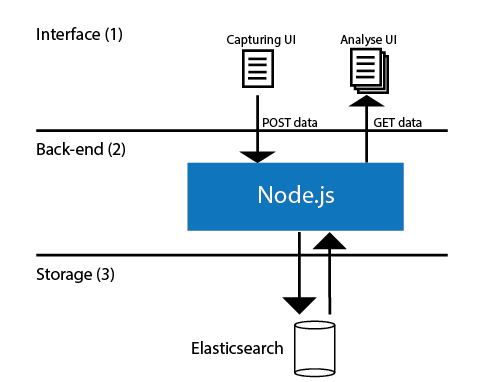
\includegraphics[width=1\textwidth]{images/architecture/architecture.png}
\caption{Overall architecture of the system }
\label{overflow}
\end{figure}

The system architecture can be layered into three layers; client (interfaces), back-end and database. The control flows from the clients requesting a page or inserting data, to the back-end, who communicates with the storage. From the storage, the execution cycle is reversed. The storage will execute what it’s been asked to do by the back-end and return the result. The back-end then again returns the result to the client.

\subsection{Interfaces (1)}

The Soccer Analytic tool has one user interface - the web browser interface. Both the capturing and the analytic interfaces can be reached from this single web browser interface running on the same domain. All interfaces are created on the client with client-side scripting using JavaScript. The client will get data from the back-end and construct the interfaces dynamically, typical for Single Page Application's\cite{SPA}.

\subsection{Back-end (2)}

The back-end is the middle layer between the client and the storage. Its main task is to serve static files to the clients, handle data insertions or handling web request by mapping them to database operations. New data insertions are possible inserted into several database indexes. The back-end will then ensure that all indexes are updated before returning success to the client. 

\subsection{Storage (3)}

The storage layers task is to persist data and handle search queries on the data. It consists of several indexes that each stores a part of the domain model. The storage will get requests over \ac{HTTP}, examine and execute them, before returning a response over the HTTP connection. 

\subsection{Domain model}

The domain model is based around matches. All attacks are wrapped into a match root document as subdocuments of the match document. Inside each attack, all passes together with other information related to an attack is. This gives the end-users an easy way of understanding how all the data is related together. Below is a complete example of how it all is structured. The number of attacks and passes is stripped down to one in the example.

\lstinputlisting{domainmodel.js}
\label{list:domainmodel}

\begin{figure}[ht!]
\centering
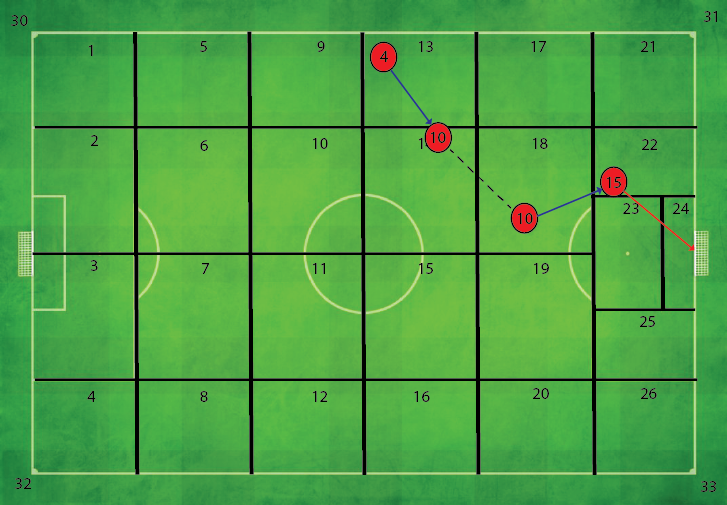
\includegraphics[width=1\textwidth]{images/general/capture_illustration.png}
\caption{The final dividing of the pitch attacking from left to right. More zones have been added to the penalty box area than the initially model. }
\label{fig:finalPitchDividing}
\end{figure}

Figure \ref{fig:finalPitchDividing} shows the final version of the pitch dividing with a illustration of how the dividing is used when storing attacks. Player 4 plays to player 10 from zone 13 to zone 14.  Player 10 transports the ball until he passes to player 15 from zone 18 to 22. Player 15 tries a finish from zone 22 inside the penalty area. The reason for going for more zones in the penalty area was a specific request by \ac{TIL} to be able to see more specific where attacks are finished from.

\section{Implementation details}

\begin{table}[ht!]
\centering
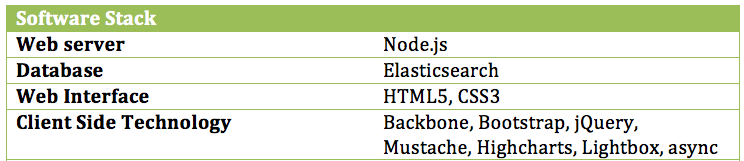
\includegraphics[width=1\textwidth]{images/implementation/software_stack.png}
\caption{Software stack}
\end{table}

\subsection{Storage}

The data storage is an Elasticsearch\footnote{http://www.elasticsearch.org/} database. Elasticsearch is document oriented, schema less and works well with \ac{JSON}\footnotemark. As our server is built on server side JavaScript, working with \ac{JSON} is easy. \ac{JSON}-objects is sent to the Elasticsearch, and will be mapped to fields and values, and made available for search in real time.
Elasticsearch takes advantages of embedded documents meaning we can store related data together. An attack is usually made up of several passes and can be stored as embedded documents wrapped in the attack document. Then all passes can be retrieved in one query when fetching an attack. Similar, retrieving a match will get all attacks and their corresponding passes in one query.

One of the main reasons for using Elasticsearch is its search capabilities. In the starting phase of the project MongoDB\footnotemark was the storage engine. However, as some aggregation queries were hard to figure out how to do, a change to Elasticsearch was made. It should be noted that MongoDB supports map reduce operations. With some extra work the queries causing problems could possible have been done with MongoDB. However, with Elasticsearch you can in a single, simple to write query get counted how many passes all players for a team has played and received, the number of times all players has been the breakthrough-player in an attack, sum type of attacks, count the most used zones for passing and finishing in the attacks and so on. This makes it very easy and efficient to do queries for analyses on teams and players.

Another feature of Elasticsearch is how easy it is to scale it by adding new nodes to your cluster. It is built to scale horizontally out of the box. Elasticsearch uses a sharding technique to spread data across the cluster.  Basically, it breaks up the data into smaller chunks spreading it across the cluster of machines to achieve scalability and performance. The configuration setup is highly adjustable letting you specify number of shards and replicas the storage shall keep. Adding a new machine to the cluster will automatically start a reorganizing process of the data to take advantage of the extra hardware. This make it suitable as our storage if we wanted to expand the project by adding more data and having more end users.

\footnotetext{http://www.json.org/}
\footnotetext{http://www.mongodb.org/}

\subsubsection{Indexes}

Indexes are much like tables in a relational database in the way that they are a container for data. An index stores documents, which is a bunch of key/value pairs, like \ac{JSON}. You can let Elasticsearch automatic analyze the field data or you can use mappings. For supporting querying on players and other fields where the value is more than one word, you have to tell Elasticsearch that it is a multi field. For example, searching for player names, which is made up of two words, when the field is not set as multi field, will give out two results and not one, as you would expect.

In our project we have 5 different indexes. 
\begin{itemize}
\item \emph{Team index}: Holds all the teams.
\item \emph{Player index}: Holds all players for every team.
\item \emph{Match index}: Holds all data from every match, including all attacks for each match.
\item \emph{Attack index}: Holds all attacks in every match.
\item \emph{Pass index}: Holds all passes in every attack.
\end{itemize}

Listing \ref{list:domainmodel} shows an example of data stored from a match. As may be noted there is data redundancy as some indexes stores the same information. One can argue that storage has become so cheap and if you can use a little bit extra space to gain performance you would do it. In this case it was done to be able to fully support aggregation functions on subdocuments explained in more details in section \ref{sec:facets}

\subsection{Facets}
\label{sec:facets}
Doing searches in Elasticsearch returns documents that matches your query. Facets provide an ability to do aggregation functions on the result-documents from your query. In the system, this feature is used a lot. An example is a query on all attack documents matching a team name. After fetching every document, aggregation functions will run on the resulting set of documents. This includes counting the number of times a player has been the sender and receiver of a pass, number of times he has been the breakthrough player, sum the type of attacks to mention a few. 

Elasticsearch will return the whole root document when you do a match query on a field in a subdocument. Since attacks for both teams are stored inside the same match document, we would get both teams attacks when doing a match query on a attack subdocument. This would again lead to aggregation functions running on both teams attack, something that would not be correct. Therefor, we have some data redundancy in our database by having multiple indexes.

Another solution to avoid data redundancy would be to store attacks for a team in a own match document. This would lead to a little more complex query when fetching matches, but save us from storing duplicated attacks and passes. If this were to be implemented again, it would most likely have been the solution.

\subsection{Back-end}

\subsubsection{Overview}	
The back-end is the middleware between the clients and the data layer and is written in Node.js\cite{node.js} It exposes a \ac{REST}\footnote{http://www.ibm.com/developerworks/webservices/library/ws-restful/} interface over \ac{HTTP} shown in figue \ref{fig:api} for the client to communicate. A request coming in is transformed to a database query based on the resource (URL) it tries to access. Node.js is a packaged compilation of Googles JavaScript engine\footnote{https://code.google.com/p/v8/} engine. It’s a relatively new (being released in 2009) and unproven platform, but has gained a lot of hype in the computer science community for its lightweight and efficient model. This comes from the even-driven and non-blocking I/O model. Per default, an instance of node runs in a single thread and does not utilize other CPU cores. When writing a web server with Node.js, you need to avoid long, blocking computations as this will block the node process for handling new incoming requests. Our back-end uses non-blocking I/O calls when accessing the database to avoid this issue.

The back-end takes use of several node packages\footnote{https://npmjs.org/}, including the Express framework, which is a web framework. 

\subsubsection{Routing}

The web server code is structured up in modules. For example requests on the URL /players is routed to the Player module for further handling. Similar, you have an attack module, pass module, team module, player module and a match module. A very often used URL is /team/:name. A \ac{HTTP} GET on this URL will be routed to the team module where a query for information about the specified team is run. On answer from the database, the result is transformed before returning it to the client. 

Similar, if the client sends new data for a match the server will insert the data into the appropriate indexes. The server will respond will HTTP status code 201 if all goes well or 400 on an error. The server uses \ac{HTTP} code actively to tell the client the result of a request. For all \ac{HTTP} POST requests the server will send status code 201, meaning that a new resource is created. For \ac{HTTP} GET requests the server responds as normal with status code 200, if all went well. 

No URL route uses \ac{HTTP} PUT and DELETE methods. These methods could have been used for deleting or updating attacks or passes. Typically, an operator will do a mistake while capturing new attacks, and then these HTTP methods would be naturally to use to update or delete data.

In principle, since the data input is generated in the web browser (with JavaScript), it could have been inserted right away into the database because of Elasticsearchs \ac{CRUD} API\footnote{http://www.elasticsearch.org/guide/en/elasticsearch/reference/current/docs.html}.  Having the server API we can hide details from the client as combining multiple queries, joining and cleaning of data. Normally, you validation of the data at the back-end is done before inserting into to the database. The client also needs to get the client code from somewhere. Therefor, having a web server was the chosen way to go.

\subsubsection{API}

The \ac{API} of the web server is listed in figure \ref{fig:api}. As mentioned the \ac{API} follows the basic \ac{REST} principles using the URL as a resource identifier and HTTP methods like GET and POST to specify actions to be taken on the resource.

\begin{table}[ht!]
\centering
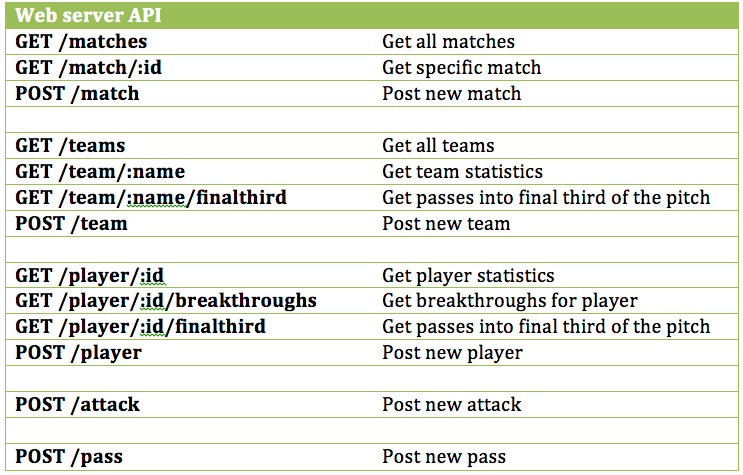
\includegraphics[width=1\textwidth]{images/implementation/API.png}
\caption{Overview of the web servers API}
\label{fig:api}
\end{table}

\subsection{Client and interfaces}

The front end is a \ac{SPA} using Backbone.js\footnotemark as under-supporting library. Having a \ac{SPA} model means that not every code is necessary loaded at once (\ac{HTML}, \ac{CSS} and JavaScript), but when needed. Also, the whole page does not reload when users navigate around, only parts of it will be updated. This is all possible because of \ac{AJAX}, a way for JavaScript running in a browser to make HTTP requests to back-end web servers. It’s asynchronously, meaning that the web page is still responsive and navigable during the request\cite{ajax}.

Backbone uses a \ac{MVP} model to structure the code. With Backbone your views will update automatic when data changes. You use Backbones models and presenters (called views in the documentation of Backbone) by letting your own models and presenters inherit Backbones basic classes. Figure \ref{fig:backbone_architecture} shows how the overall architecture of the front-end. In the following sections the architecture of the client and how different concepts in Backbone is used will be described. 

\footnotetext{http://backbonejs.org/}

\begin{figure}[ht!]
\centering
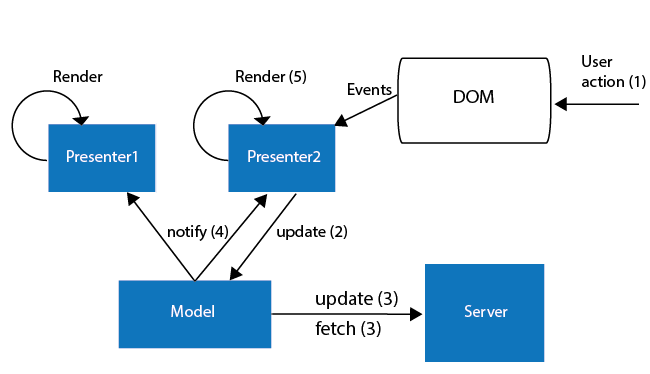
\includegraphics[width=1\textwidth]{images/architecture/backbone_architecture.png}
\caption{Architecture of the client side. Numeration is used in the text to reference the figure}
\label{fig:backbone_architecture}
\end{figure}

\subsubsection{Models}

In Backbone you encapsulate data and do communication with the back-end with objects called models. A model has mainly two responsibilities; whenever an update on a models data occurs the model notifies the presenters that have subscribed for update events for that particular model (4). The second is that models are responsible for \ac{AJAX} communication with the back-end (3). An example is when a user registers a new attack for a match. He fills out a form and press the submit button (1). Then a new attack model containing the data type in the form is created. Calling save on the model will send an \ac{AJAX} post request to the server with the models data in the \ac{HTTP} body (3).

Similar to an attack model, we have player models that handles everything around a player. When a user navigate to a players profile, the model will fetch statistics from the back-end (3) and notify the presenter that the data is ready (4), and the \ac{HTML} will be rendered in the web browser.

There is also a match model for fetching and registration of matches, team model for viewing statistics, and a pass model for saving passes. They work it the same way as the models described above using \ac{AJAX} to communicate with the back-end and notification presenters on data changes.

\subsubsection{Collections}
Collections are a set of Backbone models. It has almost the same functionality as a model. You can bind functions to happen on events for any model in the collection. On the client there is two places where collections are used; players and teams page. Naturally, players contain many player models and teams collections contain many team models.

\subsubsection{Presenters}

Presenters are the glue between the Backbone models and the view (web page).  Presenters can bind own functions to respond to models events. For example on data change event from a model the presenter will call its render function and the \ac{UI} will be updated (4). Each presenter has a own \ac{HTML} div tag which it inserts HTML to. Including to subscribing to events on models, the presenter can subscribe for view events that happens in the \ac{DOM}, events that the user triggers (1). Following up the example in the previous section on an attack registration; when a user press the submit button the presenter will be notified. He will create a model for the attack and call the save method on the instance object. 

On initialization of a presenter object it is initialized with a model or a collection depending on the view it should render.  After the model/collection has fetched its data the presenters render function will be called. This is where the data is inserted into the \ac{HTML} template (5) explained in more details in the next sections. Which event a presenter should listen to on a model is also set up when initializing a presenter.

\subsubsection{Views}

For an analytic toolkit to be useful a good presentation is critical. Here several helper libraries are used to present the data. Highcharts.js\footnotemark is a JavaScript library for illustrating statistics. A query on team generates a lot of statistics and rather than listing them up they are presented using charts. Using charts gives us the advantage of displaying several numbers for each player by plotting it in the same graph. In figure \ref{fig:chart} the number of times a player has been involved in all attacks, the number of passes into the final third of the pitch and the number of times a player has been the breakthrough-player is shown.

\footnotetext{http://www.highcharts.com/}

\begin{figure}[ht!]
\centering
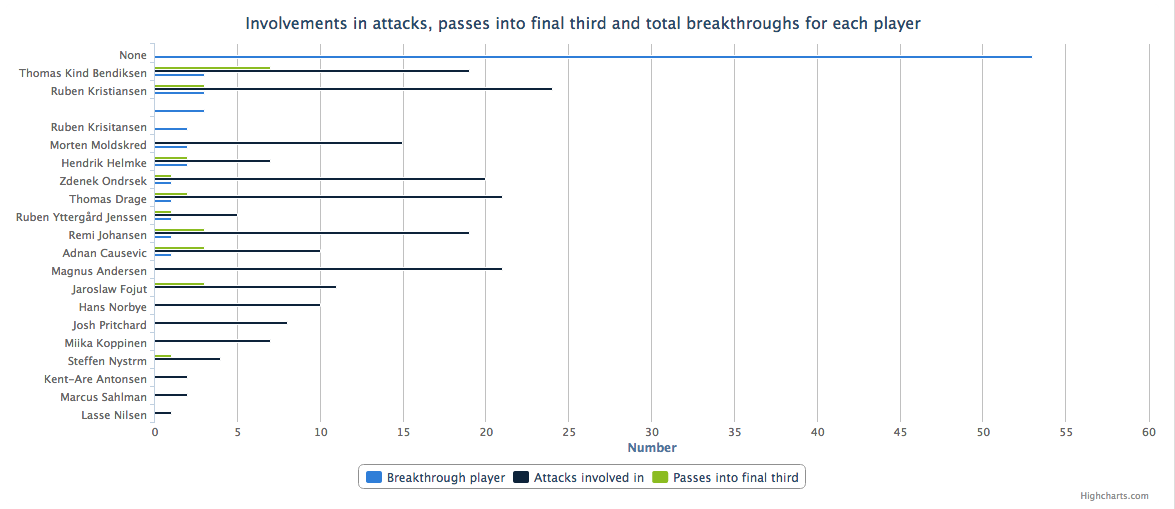
\includegraphics[width=100mm]{images/general/chart_passes.png}
\caption{Shows how statistic is illustrated on the client by using Highcharts.js.}
\label{fig:chart}
\end{figure}

To display statistics as where attacks have been finished from, we are using the \ac{HTML} canvas element. It lets you draw graphics on the fly in the web page. In this system it is used to create an element that symbols the different zones in our domain model by drawing a soccer pitch with the all the zones plotted. The team model will fetch data from the back-end containing numbers for all zones. This is then plotted into the respective zones on the pitch as figure \ref{fig:attacking_zones} is showing.

\begin{figure}[ht!]
\centering
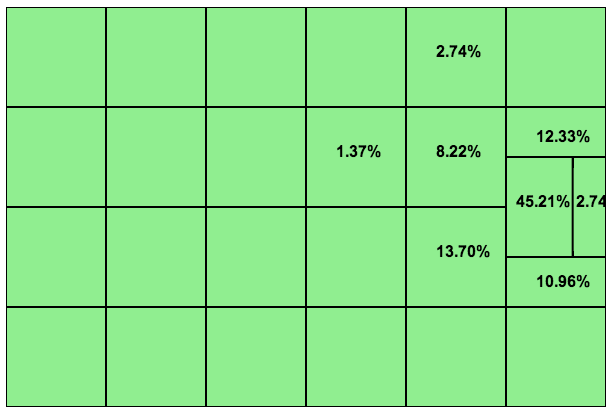
\includegraphics[width=85mm]{images/general/finishing_zones.png}
\caption{ Illustrates which zones \ac{TIL} has finished their attacks from in percent. }
\label{fig:attacking_zones}
\end{figure}

Backbone comes with a library Underscore.js\footnotemark that makes creating HTML pages with dynamic content easy. When you are rendering new content on the site you can insert data retried from a model dynamically into the HTML. This is the presenters responsibility (5). In the example below the input is a an array of objects where each element in the array contains a key value pair 'name' : value. The HTML output of this will be a list of all player names in the array. 

\lstinputlisting{underscore_example.html}
\footnotetext{http://underscorejs.org/}

\subsubsection{Router}

A component not mentioned before is the router. The router is the glue that binds all the other Backbone modules together. It handles the navigation between pages in the application. When users navigate on the page by clicking on links or buttons in a traditional web page the back-end serves a new HTML page. Here, a router module handles this click event. The router model examines the URL request and routes the request to the presenter responsible for that specific route. This is mapped inside the router. The presenter will then call fetch functions on the model to get data from the back-end and render the HTML to its assigned DIV.

The header on the page is static and will only be rendered once when the user first visits the web page. 

\subsection{Building the database, players and teams}

Finding squads in a useful format like \ac{XML} or \ac{JSON} was harder than expected. On the Norwegian football alliance's website you could download the squads for the current season, but only in PDF format. Current squads is fetched from altomfotball.no, a website by the Norwegian broadcasting company TV2. The fetching process is an own python script meant to run only once to set up the database. For each team the script basically reads the HTML document with all players listed, parse out players name, and sends in to the web server.

\subsection{Security}
Security is not taken into concern in the system. This means anyone getting into the page can post new match data and add attacks. This could have been fixed by requiring a login before getting access to the site. 







